\documentclass[main]{subfiles}
\begin{document}
\chapter{ポールを周回しながら人が近づくと威嚇する}

これは最終課題5「警備員」の課題です。

\section{課題概要}
ロボットはポールを中心とした半径50cmの円を反時計回りに周回する。
ポールの直径は約12cm。
初期位置の制約は定められていないので、
前方もしくは左方にポールを見るような地点ならば
任意の場所からスタート可能なように設計を行った。
周回中にセンサが人に反応した場合、人とポールの間に立ち威嚇を行う。
威嚇時の動作は定められていなかったので、
ポールから2m以内の範囲で追いかける設計とした。
センサが人を捉えられなくなったり、ポールから2m以上離れてしまった場合は
再びポールの周回に戻る。

\section{解法}
物体認識やそれに伴う時間に依存しない(つまり次のサイクルに持ち越される)
同一物体判定など複雑な処理が多く、また要求される動作の種類もある程度の数が予想できたので、
現在の状態を表す変数\textit{robostate}を作成し、
ロボットの動作が以下の図のように状態遷移していくような設計にした。
\begin{figure}[H]
	\centering
	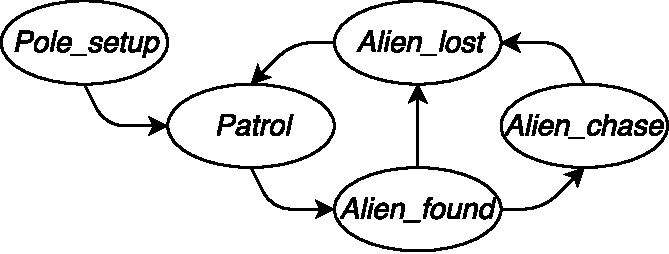
\includegraphics{img/guard_state.pdf}
	\caption{作成したプログラムの状態遷移}
\end{figure}

\subsection{共通}

\subsection{ポールの探索}
状態遷移図では\textit{Pole\_setup}に対応する。

全状態で唯一GL座標を基準に動作する。
\subsection{パトロール}
状態遷移図では\textit{Patrol}に対応する。

\subsection{不審者発見}
状態遷移図では\textit{Alien\_found}に対応する。

\subsection{不審者追従}
状態遷移図では\textit{Alien\_chase}に対応する。

\subsection{不審者逃走}
状態遷移図では\textit{Alien\_lost}に対応する。

戻ってくる。

\section{結果}
\section{考察}

\end{document}
